\documentclass[11pt]{article}

\usepackage[a4paper,margin=1in]{geometry}
\usepackage[T1]{fontenc}
\usepackage[utf8]{inputenc}
\usepackage{lmodern}
\usepackage{microtype}
\usepackage{amsmath,amssymb,bm}
\usepackage{booktabs,array,longtable,tabularx}
\usepackage{enumitem}
\usepackage{xcolor}
\usepackage{graphicx}
\usepackage{hyperref}
\usepackage{tikz}
\usetikzlibrary{arrows.meta,positioning,calc,shapes.geometric,fit,backgrounds}
\usepackage{listings}
\usepackage{caption}
\usepackage{float}
\newcolumntype{L}[1]{>{\raggedright\arraybackslash}p{#1}}
\newcolumntype{Y}{>{\raggedright\arraybackslash}X}

\hypersetup{
  colorlinks=true,
  linkcolor=blue!50!black,
  citecolor=blue!50!black,
  urlcolor=blue!50!black
}

\lstdefinestyle{code}{
  basicstyle=\ttfamily\small,
  columns=fullflexible,
  breaklines=true,
  frame=single,
  framerule=0.3pt,
  backgroundcolor=\color{black!2},
  xleftmargin=0.5em,
  xrightmargin=0.5em
}
\lstset{style=code}

\setlength{\emergencystretch}{2em}
\setlist[itemize]{leftmargin=*}
\setlist[enumerate]{leftmargin=*}

\newcommand{\CQ}{C_Q}
\newcommand{\Vzz}{V_{zz}}
\newcommand{\etaEFG}{\eta}
\newcommand{\Tr}{\operatorname{Tr}}
\newcommand{\dd}{\mathrm{d}}
\newcommand{\ee}{\mathrm{e}}
\newcommand{\RMT}{R_{\mathrm{MT}}}

\title{DFT for Spin-Dynamics Users\\
\large A Beginner-Oriented Technical Note on DFT-Derived Solid-State Parameters, with EFG Tensors as a Running Example}
\author{Technical note for the MRSpinDynamics simulation package}
\date{\today}

\begin{document}
\maketitle

\begin{abstract}
Density-functional theory (DFT) is often used upstream of a spin-dynamics simulation.  It can relax structures, compare polymorph energies, compute charge and spin densities, predict band structures and density of states, calculate vibrational modes called phonons, estimate dielectric and elastic response, and provide local spin-Hamiltonian tensors such as electric-field-gradient (EFG), magnetic-shielding, hyperfine, and sometimes spin-spin coupling tensors.  This note is written for readers with nuclear magnetic resonance (NMR), nuclear quadrupole resonance (NQR), magnetic resonance imaging (MRI), or electrical-engineering simulation backgrounds who may be new to electronic-structure calculations.  The emphasis is practical: what DFT is trying to calculate, how the self-consistent-field (SCF) loop works, how common numerical methods differ, why structure relaxation and phonons matter, what software ecosystems exist, and how to think about accuracy-speed trade-offs.  The EFG tensor and its quadrupolar NMR/NQR consequences are used as the running example, but they are not the only possible DFT output of interest.
\end{abstract}

\tableofcontents

\section{From spin dynamics to electronic structure}

A spin-dynamics code usually starts from a spin Hamiltonian: an operator that determines spin energy levels and time evolution.  For magnetic-resonance simulations, users may provide chemical shifts, dipolar couplings, scalar J-couplings, hyperfine tensors, relaxation parameters, radio-frequency (RF) pulses, static magnetic fields, and sample orientation.  In nuclear quadrupole resonance (NQR) and quadrupolar nuclear magnetic resonance (NMR), an especially important term is the interaction between a nuclear quadrupole moment and the local electric-field-gradient tensor at that nucleus.  That local tensor is determined by the electronic and ionic charge distribution in the material.

DFT is therefore not a replacement for the spin simulator.  It is a materials-physics layer that turns an atomistic structure into electronic, magnetic, vibrational, and local-tensor information that a spin simulator can consume.  A structure may enter the workflow as a crystallographic information file (CIF), a VASP-style POSCAR file, an XYZ coordinate file, or a package-specific format.  A DFT run then searches for a self-consistent electronic density: roughly, the electronic ``operating point'' compatible with the atomic structure.  From that density, the code can compute many properties.

For the present package, the electric-field-gradient (EFG) tensor is a natural first running example because it maps directly into quadrupolar Hamiltonian parameters.  However, the same DFT infrastructure can support a broader family of solid-state outputs: relaxed structures, energies, charge densities, spin densities, vibrational modes called phonons, density of states (DOS), magnetic shielding tensors, hyperfine tensors, and response properties.  The note therefore begins broadly, then returns repeatedly to the EFG example.

\begin{figure}[H]
\centering
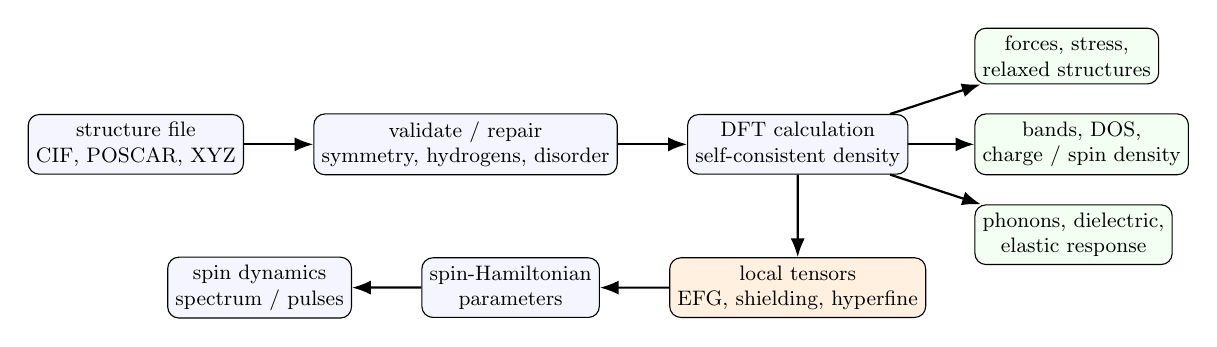
\begin{tikzpicture}[scale=0.84,transform shape,
  node distance=1.05cm,
  box/.style={draw,rounded corners,align=center,minimum width=2.35cm,minimum height=0.78cm,fill=blue!4,font=\small},
  outbox/.style={draw,rounded corners,align=center,minimum width=2.6cm,minimum height=0.78cm,fill=green!5,font=\small},
  hi/.style={draw,rounded corners,align=center,minimum width=2.6cm,minimum height=0.78cm,fill=orange!12,font=\small},
  arrow/.style={-{Latex[length=2.4mm]},thick}
]
\node[box] (structure) {structure file\\CIF, POSCAR, XYZ};
\node[box,right=of structure] (clean) {validate / repair\\symmetry, hydrogens, disorder};
\node[box,right=of clean] (dft) {DFT calculation\\self-consistent density};
\node[outbox,above right=0.45cm and 1.0cm of dft] (geom) {forces, stress,\\relaxed structures};
\node[outbox,right=1.0cm of dft] (bands) {bands, DOS,\\charge / spin density};
\node[outbox,below right=0.45cm and 1.0cm of dft] (phonons) {phonons, dielectric,\\elastic response};
\node[hi,below=1.25cm of dft] (local) {local tensors\\EFG, shielding, hyperfine};
\node[box,left=of local] (spinparams) {spin-Hamiltonian\\parameters};
\node[box,left=of spinparams] (spin) {spin dynamics\\spectrum / pulses};
\draw[arrow] (structure) -- (clean);
\draw[arrow] (clean) -- (dft);
\draw[arrow] (dft) -- (geom);
\draw[arrow] (dft) -- (bands);
\draw[arrow] (dft) -- (phonons);
\draw[arrow] (dft) -- (local);
\draw[arrow] (local) -- (spinparams);
\draw[arrow] (spinparams) -- (spin);
\end{tikzpicture}
\caption{A broad view of DFT in a spin-dynamics workflow.  EFG tensors are highlighted because they are the running example, not because they are the only useful DFT output.}
\label{fig:broad-workflow}
\end{figure}

\subsection{Typical DFT outputs relevant to magnetic-resonance simulations}

\begin{table}[H]
\centering
\small
\begin{tabularx}{\textwidth}{L{0.22\textwidth}Y Y}
\toprule
\textbf{Output class} & \textbf{Examples} & \textbf{Why a spin-dynamics user might care} \\
\midrule
Structure and energetics & Total energy, formation energy, polymorph ranking, forces, stress, optimized coordinates, equation of state & Choose the correct polymorph or protonation state; relax hydrogen positions; estimate whether a proposed defect or molecular conformation is plausible. \\
Electronic structure & Band structure, density of states (DOS), band gap, Fermi surface, charge density, electrostatic potential & Decide whether the material is insulating or metallic; understand convergence difficulty; identify charge-transfer or bonding motifs that influence local tensors. \\
Magnetism & Spin density, local magnetic moments, exchange constants from energy mapping, spin-orbit coupling (SOC), magnetic anisotropy & Build spin models, estimate hyperfine terms, check whether a nonmagnetic calculation is physically inconsistent. \\
Response and dynamics & Phonons, Born effective charges that connect atomic displacement to polarization, dielectric tensors, elastic constants, molecular dynamics (MD) trajectories & Estimate finite-temperature effects, phonon averaging, strain sensitivity, and dynamic disorder that can broaden or shift spectra. \\
Local spin-Hamiltonian tensors & EFG tensors, shielding tensors, chemical-shift tensors after referencing, hyperfine tensors, electron $g$ tensors, J-coupling tensors when implemented & Provide direct input to NMR, NQR, electron paramagnetic resonance/electron spin resonance (EPR/ESR), muon-spin, or related spin-dynamics calculations. \\
\bottomrule
\end{tabularx}
\caption{DFT can produce many outputs.  Not every code implements every property, and not every property has the same accuracy requirements.}
\label{tab:dft-outputs}
\end{table}

The rest of the note follows the same logic as the workflow diagram.  First we define the EFG running example, because it is the property most directly tied to NQR frequencies.  Then we step backward to the electronic-structure calculation that produces the density, the numerical methods used to solve it, and the structural/thermal approximations that often control the error.

\section{The running example: EFG tensors and quadrupolar frequencies}

\subsection{Definition}

The electric potential $\Phi(\mathbf r)$ at a point in a solid is produced by electrons and ions.  The electric field is the first derivative of the potential, and the electric-field gradient is the second derivative evaluated at a nuclear site $A$:
\begin{equation}
V_{ij}^{(A)} = \left.\frac{\partial^2 \Phi(\mathbf r)}{\partial x_i\,\partial x_j}\right|_{\mathbf r=\mathbf R_A}.
\label{eq:efgdef}
\end{equation}
Some codes use the opposite sign because they define the EFG as a derivative of the electric field rather than of the electrostatic potential.  This sign convention matters when tensor orientations are combined with Zeeman terms, meaning static magnetic-field interactions, or with RF fields.  It matters less for a pure zero-field NQR search in which only absolute transition frequencies are used.

In the usual convention, the EFG tensor is symmetric and traceless:
\begin{equation}
V_{ij}=V_{ji}, \qquad \Tr(\mathbf V)=V_{xx}+V_{yy}+V_{zz}=0.
\end{equation}
It can be diagonalized to obtain its principal-axis frame.  A common NMR/NQR convention orders principal components as
\begin{equation}
|V_{zz}| \ge |V_{yy}| \ge |V_{xx}|,
\end{equation}
and defines
\begin{equation}
\etaEFG = \frac{V_{xx}-V_{yy}}{V_{zz}}, \qquad 0 \le \etaEFG \le 1 .
\label{eq:eta}
\end{equation}
Code manuals do not always use the same ordering or sign convention.  A robust parser should therefore store the full tensor, the principal values, the eigenvectors, the ordering convention, and the units.  Reducing everything to a scalar frequency too early loses important information.

\begin{figure}[H]
\centering
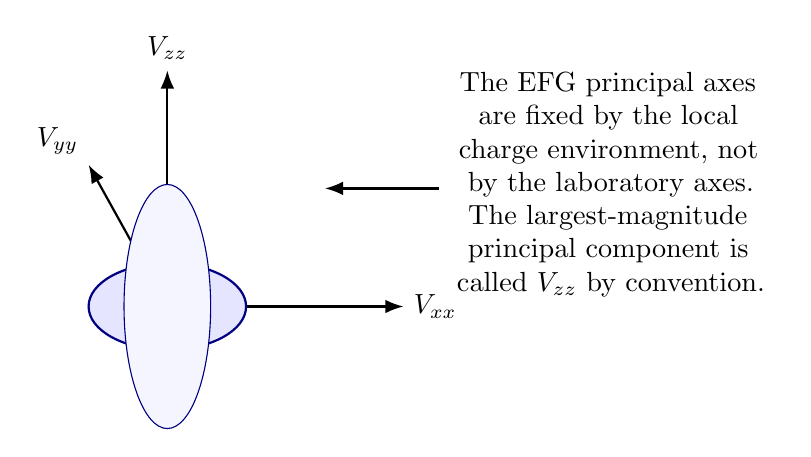
\begin{tikzpicture}[scale=1.0,>=Latex]
  \draw[thick,->] (0,0) -- (3,0) node[right] {$V_{xx}$};
  \draw[thick,->] (0,0) -- (-1.0,1.8) node[above left] {$V_{yy}$};
  \draw[thick,->] (0,0) -- (0,3.0) node[above] {$V_{zz}$};
  \draw[fill=blue!10,draw=blue!50!black,thick] (0,0) ellipse (1.0 and 0.55);
  \draw[fill=blue!4,draw=blue!50!black] (0,0) ellipse (0.55 and 1.55);
  \node[align=center,text width=4.2cm] at (5.6,1.55) {The EFG principal axes are fixed by the local charge environment, not by the laboratory axes.  The largest-magnitude principal component is called $V_{zz}$ by convention.};
  \draw[->,thick] (3.45,1.5) -- (2.0,1.5);
\end{tikzpicture}
\caption{Cartoon of an EFG principal-axis frame.  The ellipses are a visual metaphor for local anisotropy, not literal charge-density surfaces.}
\label{fig:efgaxes}
\end{figure}

\subsection{From EFG to a quadrupolar Hamiltonian}

For a nucleus with spin $I>1/2$ and electric quadrupole moment $Q$, the quadrupole coupling constant is commonly written as
\begin{equation}
\CQ = \frac{e Q V_{zz}}{h},
\label{eq:cqdef}
\end{equation}
where $e$ is the elementary charge and $h$ is Planck's constant.  A useful unit conversion is
\begin{equation}
\CQ[\mathrm{MHz}] \simeq 24.1799\, Q[\mathrm{barn}]\,
\left(\frac{V_{zz}}{10^{21}\,\mathrm{V/m^2}}\right).
\label{eq:unitconv}
\end{equation}
Equivalently, $1\,\mathrm{V}/\text{\AA}^{2}=10^{20}\,\mathrm{V/m^2}$.

In the EFG principal-axis frame, a common quadrupolar Hamiltonian convention is
\begin{equation}
\frac{\mathcal H_Q}{h}=
\frac{\CQ}{4I(2I-1)}
\left[3\hat I_z^2-I(I+1)+\etaEFG(\hat I_x^2-\hat I_y^2)\right],
\label{eq:hq}
\end{equation}
where the spin operators are dimensionless.  A spin-dynamics simulator should ideally reconstruct $\mathcal H_Q$ from the full EFG tensor and nuclear $Q$ rather than from only $\CQ$ and $\etaEFG$, because tensor orientation matters in oriented samples, powder averaging, mixed Zeeman-quadrupole regimes, strain-dependent simulations, and pulse calculations.

For common zero-field examples,
\begin{align}
I=\frac{3}{2}:\quad
\nu_{\mathrm{NQR}} &= \frac{|\CQ|}{2}\sqrt{1+\frac{\etaEFG^2}{3}},
\label{eq:spin32freq}\\[3pt]
I=1:\quad
\nu_+ &= \frac{|\CQ|}{4}(3+\etaEFG),\qquad
\nu_- = \frac{|\CQ|}{4}(3-\etaEFG),\qquad
\nu_0 = \frac{|\CQ|}{2}\etaEFG .
\label{eq:spin1freqs}
\end{align}
For $I=1$, the three transition frequencies obey $\nu_+=\nu_-+\nu_0$.

\section{DFT in one page}

To understand where DFT outputs come from, start with one physical approximation.  In the Born-Oppenheimer approximation, the nuclei are treated as fixed while the electrons adjust to those nuclear positions.  The full many-electron Schrodinger equation for those electrons is still too large to solve directly for most solids.  Density-functional theory (DFT) replaces the many-electron wavefunction by the electron density $n(\mathbf r)$ as the central variable.

The practical Kohn-Sham formulation maps the interacting-electron problem onto a set of effective one-electron equations,
\begin{equation}
\left[-\frac{\hbar^2}{2m_e}\nabla^2 + V_{\mathrm{eff}}[n](\mathbf r)\right]\psi_i(\mathbf r)
= \varepsilon_i\psi_i(\mathbf r),
\label{eq:ks}
\end{equation}
where
\begin{equation}
V_{\mathrm{eff}}[n] = V_{\mathrm{ion}} + V_{\mathrm{Hartree}}[n] + V_{\mathrm{xc}}[n].
\end{equation}
Here $V_{\mathrm{ion}}$ is the ionic potential, $V_{\mathrm{Hartree}}$ is the classical electron-electron electrostatic potential, and $V_{\mathrm{xc}}$ is the exchange-correlation (XC) potential.  The XC functional is where much of the physics approximation lives.  Common choices include the local-density approximation (LDA), generalized-gradient approximation (GGA) functionals such as Perdew-Burke-Ernzerhof (PBE), solid-optimized GGAs such as PBEsol, meta-GGAs, dispersion-corrected functionals for van der Waals interactions, DFT+$U$ corrections for localized $d$ or $f$ electrons, and hybrid functionals that include a fraction of exact exchange.

For an NMR/NQR user, the key point is not that DFT gives ``the wavefunction.''  The practical key is that DFT gives a self-consistent electronic charge density, spin density, total energy, forces on atoms, stress on the cell, and related response quantities.  The EFG is then obtained from the second derivative of the electrostatic potential created by that self-consistent density and by the ions.  Other spin-Hamiltonian parameters are obtained from other derivatives or response calculations built on the same electronic ground state.

\section{The SCF loop and the DC operating-point analogy}

The Kohn-Sham equations depend on $n(\mathbf r)$, but $n(\mathbf r)$ is built from their solutions:
\begin{equation}
 n(\mathbf r)=\sum_i f_i |\psi_i(\mathbf r)|^2,
\end{equation}
where $f_i$ are orbital occupancies.  DFT therefore solves a nonlinear fixed-point problem.  A typical self-consistent-field loop is:
\begin{enumerate}
\item Guess an initial density, often a superposition of neutral atomic densities.
\item Build $V_{\mathrm{eff}}[n]$.
\item Solve the Kohn-Sham eigenvalue problem.
\item Recompute $n(\mathbf r)$ from the occupied states.
\item Mix the new density with the old density to improve stability.
\item Repeat until the energy, density residual, forces, and target properties are converged.
\end{enumerate}

This is closely analogous to a DC operating-point calculation in SPICE.  In a nonlinear circuit, device currents depend on node voltages, while node voltages are determined by Kirchhoff equations containing those currents.  A simulator iterates until currents and voltages are mutually consistent.  In DFT, the potential depends on the density, while the density is determined by the potential.  DFT convergence failures often feel familiar to circuit simulators: poor initial guesses, unstable mixing, metallic states with sharp occupancy changes, competing magnetic states, or an ill-conditioned problem can cause slow convergence or oscillation.

\begin{figure}[H]
\centering
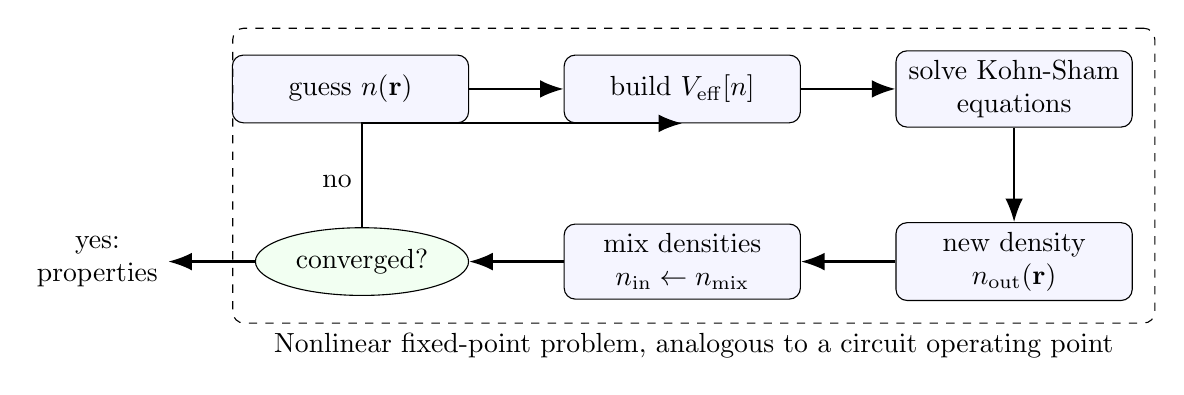
\begin{tikzpicture}[
  node distance=1.2cm,
  box/.style={draw,rounded corners,align=center,minimum width=3.0cm,minimum height=0.86cm,fill=blue!4},
  circ/.style={draw,ellipse,align=center,minimum width=2.5cm,minimum height=0.86cm,fill=green!5},
  arrow/.style={-{Latex[length=3mm]},thick}
]
\node[box] (guess) {guess $n(\mathbf r)$};
\node[box,right=of guess] (pot) {build $V_{\mathrm{eff}}[n]$};
\node[box,right=of pot] (solve) {solve Kohn-Sham\\equations};
\node[box,below=of solve] (density) {new density\\$n_{\mathrm{out}}(\mathbf r)$};
\node[box,left=of density] (mix) {mix densities\\$n_{\mathrm{in}} \leftarrow n_{\mathrm{mix}}$};
\node[circ,left=of mix] (conv) {converged?};
\draw[arrow] (guess) -- (pot);
\draw[arrow] (pot) -- (solve);
\draw[arrow] (solve) -- (density);
\draw[arrow] (density) -- (mix);
\draw[arrow] (mix) -- (conv);
\draw[arrow] (conv.north) |- node[pos=0.22,left] {no} (pot.south);
\draw[arrow] (conv.west) -- ++(-1.1,0) node[left,align=center] {yes:\\properties};
\node[draw,dashed,rounded corners,fit=(pot)(solve)(density)(mix)(conv),inner sep=0.28cm,label=below:{Nonlinear fixed-point problem, analogous to a circuit operating point}] {};
\end{tikzpicture}
\caption{The self-consistent-field loop.  A post-SCF property such as an EFG is meaningful only after the density is converged tightly enough for the property.}
\label{fig:scf}
\end{figure}

Once the SCF loop has converged, the calculation has found a mutually consistent density and potential for the chosen structure and numerical settings.  The next question is how the continuous equations are represented on a computer.  That is where most differences between DFT codes enter.

\section{From equations to numbers: major solution methods}

DFT is not one numerical method.  The same Kohn-Sham equations can be discretized and solved in several ways.  The main differences are the basis set, meaning the mathematical functions used to represent orbitals and densities; the treatment of core electrons close to nuclei; the boundary conditions; and the method used to solve the nonlinear SCF problem.

\subsection{Periodic boundary conditions and k-points}

Most crystalline-solid DFT calculations use periodic boundary conditions (PBCs): the simulation cell repeats in space.  Electronic states are labelled by a wavevector $\mathbf k$ in the Brillouin zone, the primitive cell of reciprocal space.  Integrals over the Brillouin zone are approximated by a finite grid of k-points.  Small primitive cells, metals, and high-accuracy tensor properties usually need denser k-point sampling.  Large supercells may need fewer k-points, sometimes only the $\Gamma$ point, which is the $\mathbf k=0$ point.

For spin-dynamics users, k-points are similar in spirit to frequency-domain sampling or quadrature points.  A coarse mesh may give a plausible total energy but an unconverged local tensor.  Always converge the output quantity of interest, not only the total energy.

\subsection{Basis sets and core-electron treatments}

The basis-set choice is closely tied to how the nucleus and chemically inert core electrons are represented.  A pseudopotential replaces the bare nucleus plus core electrons by an effective potential felt by valence electrons.  An all-electron method treats core and valence electrons explicitly.  Projector augmented-wave (PAW) methods sit between these ideas: they solve a smooth pseudopotential-like problem, then reconstruct all-electron-like behavior near nuclei.  These definitions matter because EFGs are near-nuclear properties.

\begin{longtable}{@{}L{0.21\textwidth}L{0.25\textwidth}L{0.24\textwidth}L{0.22\textwidth}@{}}
\toprule
\textbf{Method family} & \textbf{Basic idea} & \textbf{Strengths} & \textbf{Cautions for EFG/local tensors} \\
\midrule
\endhead
Plane-wave pseudopotential & Expand valence wavefunctions in plane waves; replace core electrons and nucleus by an effective pseudopotential. & Systematic energy cutoff convergence; excellent for periodic solids; easy automation; fast Fourier transforms (FFTs) make electrostatics efficient. & Plain pseudopotentials without all-electron reconstruction are generally not sufficient for near-nuclear tensors.  Semicore and pseudopotential quality matter. \\
Plane-wave PAW / GIPAW & Use smooth pseudo-wavefunctions for speed, then reconstruct all-electron-like quantities near nuclei using PAW augmentation data.  Gauge-including PAW (GIPAW) extends this idea to magnetic-response calculations. & Good compromise for high-throughput solid-state NMR/NQR; common in ABINIT, VASP, GPAW, and related workflows. & Accuracy depends on PAW dataset, frozen-core approximation, augmentation radius, valence configuration, and convergence settings. \\
All-electron APW/LAPW family & Divide space into muffin-tin spheres plus an interstitial region; use radial functions near nuclei and plane waves between atoms.  APW means augmented plane wave; LAPW means linearized augmented plane wave. & High-fidelity treatment of near-nucleus quantities; strong benchmark path for EFGs, hyperfine terms, and core-sensitive properties. & Slower; more setup parameters; muffin-tin radii and linearization choices require expertise. \\
All-electron numeric atom-centered orbitals (NAOs) & Expand orbitals in numerical functions centered on atoms; treat core and valence electrons explicitly. & Accurate for molecules, surfaces, clusters, and periodic systems; basis can be made hierarchical. & Basis convergence is not a single energy cutoff; near-nuclear tensor availability depends on code implementation. \\
Localized numerical atomic orbitals with pseudopotentials & Use finite-range atomic-like orbitals and pseudopotentials. & Efficient for large systems, interfaces, and exploratory modeling. & Basis and pseudopotential transferability must be checked; near-nuclear properties need special treatment or may not be reliable. \\
Gaussian basis / molecular or periodic LCAO & Use Gaussian-type atom-centered functions, often described as a linear combination of atomic orbitals (LCAO); calculations may be all-electron or use effective core potentials. & Strong for molecular NMR, clusters, hybrid functionals, and correlated post-DFT methods; periodic versions exist. & Periodic electrostatics and basis-set superposition need care; crystal-environment effects may be lost in isolated-cluster models. \\
Real-space grids / finite differences / wavelets & Represent wavefunctions or densities directly on grids. & Flexible boundary conditions; useful for finite systems, surfaces, and adaptive accuracy. & Very fine grids may be required near nuclei unless combined with PAW or pseudopotentials. \\
Tight-binding / DFTB / machine-learned potentials & Replace parts of DFT by parameterized approximations.  DFTB means density-functional tight binding; ML means machine-learned. & Very fast; useful for structure search, molecular dynamics, and pre-screening. & Not a substitute for a converged first-principles local-tensor calculation unless carefully parameterized and validated. \\
\bottomrule
\caption{Common numerical families used in DFT and DFT-adjacent workflows.  The categories overlap: for example, PAW can be implemented with plane waves, real-space grids, or localized orbitals.}
\label{tab:method-families}
\end{longtable}

\subsection{Plane waves: why they are popular and when they struggle}

Crystals are periodic, so plane waves are a natural basis for the smooth part of the electronic wavefunction:
\begin{equation}
\psi_{n\mathbf k}(\mathbf r)=\sum_{\mathbf G} c_{n\mathbf k}(\mathbf G)\,
\ee^{i(\mathbf k+\mathbf G)\cdot\mathbf r},
\end{equation}
where $\mathbf G$ is a reciprocal-lattice vector.  The basis is controlled mainly by a kinetic-energy cutoff,
\begin{equation}
\frac{\hbar^2}{2m_e}|\mathbf k+\mathbf G|^2 < E_{\mathrm{cut}}.
\end{equation}
Increasing $E_{\mathrm{cut}}$ gives a systematic convergence path.  This is a major reason plane-wave methods are popular in automated workflows.

The challenge is that true all-electron wavefunctions oscillate rapidly near nuclei, especially for heavy atoms.  Representing those oscillations directly with plane waves would require a huge cutoff.  Plane-wave DFT therefore usually removes chemically inert core electrons and replaces the nuclear-plus-core potential with a pseudopotential or PAW dataset.  This is not a defect of DFT itself; it is a numerical strategy for making the problem tractable.

Plane waves are often less convenient for isolated molecules, large vacuum cells, localized defects requiring huge supercells, or properties dominated by core electrons.  They do not literally ``break down'' in these cases, but they can become inefficient or require additional reconstruction and correction techniques.  For EFGs, the practical rule is simple: do not trust a plain pseudopotential calculation with no all-electron reconstruction for a near-nuclear tensor property.

\subsection{PAW and GIPAW: efficient near-nucleus reconstruction}

The projector augmented-wave (PAW) method uses smooth pseudo-wavefunctions for computational efficiency, but reconstructs all-electron-like quantities inside atom-centered augmentation spheres.  This is why PAW is useful for core-sensitive properties such as EFGs and hyperfine terms.  Gauge-including PAW (GIPAW) is the corresponding framework widely used for magnetic-response properties such as NMR shielding in periodic solids.

PAW is a compromise, not magic.  It can be very accurate, but the result depends on the quality of the PAW dataset, the frozen-core approximation, whether semicore states are included as valence, and the numerical cutoff.  If two reasonable PAW datasets give materially different EFGs, the result should be treated as dataset-sensitive.

\subsection{All-electron APW/LAPW: why it is a benchmark path}

Full-potential (FP) linearized augmented-plane-wave (LAPW) methods split space into atom-centered muffin-tin regions and an interstitial region.  Inside a muffin tin, the basis is built from radial functions times spherical harmonics; in the interstitial region, plane waves are used.  The notation APW+lo means augmented plane waves plus local orbitals, a closely related basis enhancement.  No pseudopotential is required, and core and semicore electrons can be treated explicitly.  This makes FP-LAPW/APW+lo methods strong reference choices for near-nuclear observables.

The trade-off is cost and expertise.  Instead of only choosing an energy cutoff and a k-point grid, the user must also manage muffin-tin radii, $\RMT K_{\max}$, angular-momentum cutoffs, local orbitals, core/valence separation, linearization energies, and sometimes spin-orbit settings.  These choices are not impossible, but they are less beginner-friendly than a standard plane-wave PAW workflow.

\section{From static structures to finite-temperature tensors}
\label{sec:relax-phonons}

The discussion so far has treated the atomic coordinates as given.  In practice, the structure is often the dominant uncertainty.  DFT does not only compute electronic properties at fixed coordinates; it can also move atoms, test mechanical stability, and estimate thermal motion.  Those steps are essential when the target property is a local tensor such as an EFG.

\subsection{Geometry optimization: forces and stress}

For a fixed set of nuclear coordinates, an SCF calculation gives a total energy.  It also gives forces, which are energy derivatives with respect to atomic positions, and stress, which is the derivative with respect to cell strain.  A geometry optimization, also called a structural relaxation, repeatedly performs SCF calculations, computes forces and stress, and updates atomic positions and sometimes the unit cell until the structure is mechanically balanced.

For NMR/NQR work, three relaxation policies are common:
\begin{description}
\item[No relaxation] uses the experimental coordinates as-is.  This keeps the calculation close to the measured structure but can preserve bad hydrogen positions, disorder artifacts, or limited coordinate precision.
\item[Fixed-cell internal relaxation] keeps the experimental lattice parameters and cell angles, but relaxes atomic positions inside the cell.  This is often a good first correction for X-ray structures because hydrogen positions and light-atom local geometries can strongly affect local tensors.
\item[Full cell-and-atom relaxation] relaxes both atomic positions and the unit cell.  This is internally consistent for the chosen functional and pressure, but the result may resemble a zero-temperature theoretical structure rather than the finite-temperature experimental structure.
\end{description}

The best choice depends on the question.  For assigning a room-temperature NQR line, a fixed-cell relaxation of a room-temperature structure may be more relevant than a fully relaxed 0 K cell.  For comparing polymorphs or testing whether a proposed structure is mechanically reasonable, full relaxation is often necessary.

\subsection{Phonons: vibrations around a structure}

A phonon is a quantized normal mode of vibration in a crystal.  Classically, it is a collective pattern in which atoms move together at a particular frequency.  In the harmonic approximation, the energy near a relaxed structure is approximated by a quadratic function of the atomic displacements.  The second derivatives of the energy form force constants, and the mass-weighted force-constant matrix is the dynamical matrix.  Diagonalizing the dynamical matrix gives phonon frequencies and displacement patterns.

Phonons are useful for at least four reasons in a spin-dynamics workflow:
\begin{enumerate}
\item They reveal whether a relaxed structure is dynamically stable.  Imaginary phonon frequencies usually indicate that the structure wants to distort along a softer mode, or that the numerical setup is not converged.
\item They estimate zero-point motion and finite-temperature atomic displacements, both of which can average local tensors.
\item They connect to dielectric response, infrared and Raman spectra, Born effective charges, and electron-phonon effects in codes that implement the needed response theory.
\item They provide physically motivated distorted structures for tensor averaging, rather than arbitrary random coordinate noise.
\end{enumerate}

\subsection{How phonons are computed: finite displacements and DFPT}

There are two common first-principles routes to phonons:
\begin{description}
\item[Finite-displacement supercells] displace atoms slightly in a supercell, run force calculations, and estimate force constants by numerical derivatives.  This approach is conceptually simple and works with many DFT codes.  The trade-off is that many displaced structures may be needed, especially for low-symmetry or large cells.
\item[Density-functional perturbation theory (DFPT)] solves a linear-response problem around the converged ground-state density.  Instead of manually displacing atoms one by one, DFPT computes the first-order electronic response to a perturbation such as an atomic displacement, electric field, or strain.  DFPT can be very efficient and can directly access phonons at chosen wavevectors, dielectric tensors, and Born effective charges when implemented.
\end{description}

Finite differences are not limited to phonons.  The same idea can estimate derivatives of EFGs with respect to strain, electric field, atomic displacement, or defect configuration.  DFPT is the more elegant route when the relevant response is implemented; finite differences are often the more universal route when it is not.

\subsection{ABINIT's derivative database: DDB, MRGDDB, and ANADDB}

ABINIT has a useful code-specific way to organize response calculations.  A \emph{Derivative DataBase} (DDB) is an ABINIT file that stores derivatives of the total energy computed by response-function calculations.  In the ABINIT documentation, second derivatives of the total energy are often abbreviated as 2DTEs, and some third derivatives are abbreviated as 3DTEs.  These derivatives may correspond to atomic-displacement perturbations, electric-field perturbations, strain perturbations, and selected higher-order combinations.  In practical terms, the DDB is a compact record of the response information from which many phonon and material-response quantities are later derived.\cite{ABINIT_RESPFN,ABINIT_DFPTTopic}

ANADDB, short for \emph{Analysis of Derivative DataBase}, is the ABINIT post-processing program that reads a DDB and turns the stored derivatives into physical results.  Depending on which derivatives are present and which ANADDB input flags are used, it can produce interatomic force constants, phonon spectra and bands, dielectric tensors, Born effective charges, elastic and piezoelectric quantities, thermodynamic functions, and related response outputs.  MRGDDB is the companion merge utility used when DDB pieces from several perturbations or wavevectors must be combined before analysis.\cite{ABINIT_ANADDB,ABINIT_PHONONS}

For a spin-dynamics package, this distinction matters.  An ABINIT phonon or dielectric workflow is not just ``run DFT and parse one number.''  It is usually a chain: converge the ground-state SCF calculation, run DFPT datasets for the needed perturbations, collect the resulting DDB information, optionally merge DDB files with MRGDDB, analyze the result with ANADDB, and then pass selected outputs into tensor averaging or spectrum simulation.  The package metadata should therefore record not only the ground-state input, but also the DDB origin, ANADDB input, q-point grid, imposed acoustic sum rule (ASR, a translational-invariance constraint) and charge-neutrality settings when relevant, and any thermal model derived from the phonons.

\subsection{Why phonons matter for EFGs and spin dynamics}

The EFG is a second derivative of the electrostatic potential at a nucleus, so it is sensitive to local geometry.  Stretching a bond, rotating a molecular group, changing a hydrogen bond, or distorting an octahedral coordination environment can change both $\Vzz$ and $\etaEFG$.  A static EFG from a single structure is therefore a snapshot, not automatically the experimentally observed finite-temperature average.

A practical thermal workflow is:
\begin{enumerate}
\item choose a reference structure and relaxation policy;
\item calculate phonon modes or run ab initio molecular dynamics (AIMD), meaning molecular dynamics in which forces come from DFT on the fly;
\item generate thermally displaced snapshots from harmonic phonons, a quasi-harmonic thermal-expansion model, an explicit disorder model, or AIMD;
\item compute the EFG tensor for each snapshot;
\item average either the tensors or the spectra, depending on the motion timescale relative to the spin dynamics.
\end{enumerate}

The last step is not just bookkeeping.  If motion is fast compared with the spin evolution, a motionally averaged tensor may be appropriate.  If motion is slow or produces multiple quasi-static environments, the spectrum may show multiple lines or broadening.  If the EFG fluctuates at relevant frequencies, it may contribute to quadrupolar relaxation.  These are spin-dynamics questions, but DFT and phonons provide the microscopic structural input.

\begin{figure}[H]
\centering
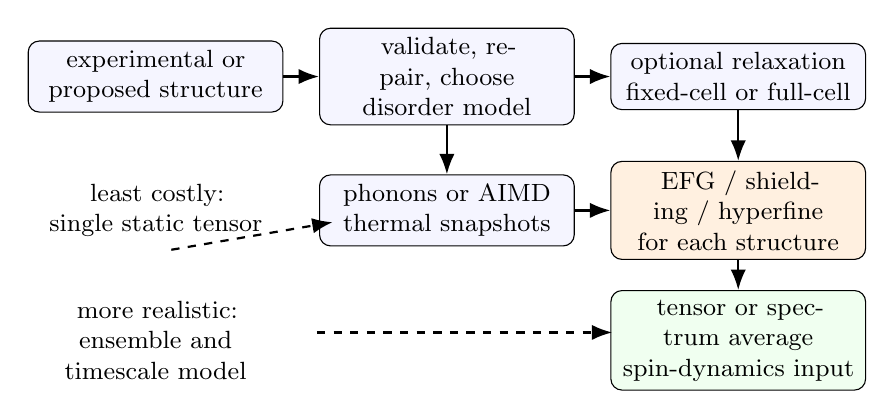
\begin{tikzpicture}[x=1cm,y=1cm,>=Latex,
  stage/.style={draw,rounded corners,align=center,font=\small,minimum height=0.78cm,text width=3.0cm,fill=blue!4},
  cost/.style={font=\small,align=center,text width=2.7cm},
  arrow/.style={-{Latex[length=2.6mm]},thick}
]
\node[stage] (cif) at (0,0) {experimental or proposed structure};
\node[stage] (fixed) at (3.7,0) {validate, repair, choose disorder model};
\node[stage] (relax) at (7.4,0) {optional relaxation\\fixed-cell or full-cell};
\node[stage] (phonon) at (3.7,-1.7) {phonons or AIMD\\thermal snapshots};
\node[stage,fill=orange!12] (efg) at (7.4,-1.7) {EFG / shielding / hyperfine\\for each structure};
\node[stage,fill=green!6] (avg) at (7.4,-3.35) {tensor or spectrum average\\spin-dynamics input};
\draw[arrow] (cif) -- (fixed);
\draw[arrow] (fixed) -- (relax);
\draw[arrow] (fixed) -- (phonon);
\draw[arrow] (relax) -- (efg);
\draw[arrow] (phonon) -- (efg);
\draw[arrow] (efg) -- (avg);
\node[cost] at (0,-1.7) {least costly:\\single static tensor};
\node[cost] at (0,-3.35) {more realistic:\\ensemble and timescale model};
\draw[arrow,dashed] (0.2,-2.2) -- (2.25,-1.85);
\draw[arrow,dashed] (2.05,-3.25) -- (5.8,-3.25);
\end{tikzpicture}
\caption{Structural fidelity ladder for tensor predictions.  The expensive steps are not always needed, but they should be considered when temperature, disorder, or motion is central to the experiment.}
\label{fig:relax-phonon-ladder}
\end{figure}

\subsection{Practical levels of structural treatment}

A useful documentation policy is to label every DFT-derived tensor by the structural model used:
\begin{enumerate}
\item \textbf{Static experimental:} CIF/POSCAR coordinates used without relaxation.  Fast, transparent, but sensitive to experimental imperfections.
\item \textbf{Hydrogen/light-atom corrected:} experimental heavy-atom framework with relaxed hydrogens or selected internal coordinates.  Often a good NMR/NQR compromise.
\item \textbf{Fixed-cell relaxed:} all internal positions relaxed at the experimental cell.  Good for local geometry while preserving measured lattice parameters.
\item \textbf{Fully relaxed:} atoms and cell relaxed.  Good for theoretical consistency and structure prediction; may shift away from finite-temperature experiment.
\item \textbf{Phonon-averaged or MD-averaged:} local tensors averaged over thermally displaced configurations.  More expensive, but necessary when thermal motion or dynamic disorder controls the spectrum.
\end{enumerate}

This section also explains why a DFT package should not report a single EFG as if it were independent of structural assumptions.  The reported metadata should record whether the structure was unrelaxed, fixed-cell relaxed, fully relaxed, phonon averaged, MD averaged, or disorder averaged.

\section{A map of common DFT codes and workflows}

The method families above become concrete through software.  A package does not need to support every DFT code, but its documentation should give users a sense of where ABINIT and Elk sit in the broader landscape and what other tools they may encounter in the literature.

\begin{longtable}{@{}L{0.14\textwidth}L{0.22\textwidth}L{0.25\textwidth}L{0.29\textwidth}@{}}
\toprule
\textbf{Code} & \textbf{Main numerical style} & \textbf{Common strengths} & \textbf{Comments for NMR/NQR/local tensors} \\
\midrule
\endhead
ABINIT & Open-source plane-wave pseudopotential and PAW code; broad DFPT capabilities & Automated periodic DFT, structural relaxation, response properties, PAW EFG calculations & Good default for scripted PAW EFG workflows.  EFG is requested after a ground-state PAW calculation; DDB/ANADDB workflows are central for phonons, dielectric, elastic, thermodynamic, and related derivative analyses. \\
Quantum ESPRESSO (QE) & Open-source plane-wave pseudopotential, ultrasoft-pseudopotential, and PAW ecosystem & Widely used periodic DFT, phonons, DFPT, materials workflows & QE-GIPAW workflows are common for NMR shielding, EFG, $g$ tensors, and hyperfine calculations, but setup depends on the specific GIPAW package and pseudopotentials. \\
VASP & Commercial plane-wave PAW code & Robust production calculations, large user base, structural relaxation, MD, many properties & Supports EFG calculations with a dedicated tag and can convert $V_{zz}$ to $\CQ$ when isotope quadrupole moments are provided.  Licensing is the main barrier for package integration. \\
CASTEP & Plane-wave pseudopotential code & Materials modeling, structural and vibrational properties, solid-state NMR tooling & Strong solid-state NMR heritage: shielding, EFG, and J-coupling workflows are documented.  Availability depends on licensing. \\
GPAW & Open-source PAW code with plane-wave, real-space grid, and LCAO modes & Python/ASE integration, flexible basis representations, good for workflow prototyping & Useful ecosystem for PAW-based calculations and custom workflows; specific local-tensor support should be checked for the desired property. \\
CP2K & Gaussian and plane-wave (GPW) mixed basis with pseudopotentials; Gaussian and augmented plane wave (GAPW) for more core-sensitive work & Large systems, condensed-phase MD, liquids, interfaces, hybrid functionals & Excellent for dynamics and large cells.  For EFGs and near-nuclear tensors, verify whether the chosen GPW/GAPW setup and property implementation are appropriate. \\
SIESTA & Pseudopotential DFT with numerical atomic orbitals & Large systems, surfaces, transport-like workflows, efficient localized basis calculations & Fast exploratory method; local tensor accuracy depends strongly on pseudopotential and basis choices and may require validation against PAW/all-electron results. \\
CRYSTAL & Periodic LCAO with Gaussian-type atom-centered functions; Hartree-Fock (HF), DFT, and hybrid functional workflows & Molecular crystals, hybrid functionals, all-electron or effective-core basis sets & Useful bridge between quantum chemistry and periodic solids; can be attractive for molecular solids and cluster/periodic comparisons. \\
FHI-aims & All-electron numeric atom-centered orbitals & Accurate molecules, clusters, surfaces, and periodic systems; systematic basis tiers & All-electron alternative to LAPW for many problems; property availability and convergence details should be checked for the desired tensor. \\
Elk & Open-source all-electron full-potential LAPW/APW+lo & Benchmark all-electron calculations, spin-orbit, magnetic and response properties & Useful high-accuracy reference path for EFGs.  Slower and more parameter-sensitive than a PAW plane-wave default. \\
WIEN2k & All-electron full-potential LAPW/APW+lo & Mature benchmark code for solids, core-sensitive properties, magnetism & Widely used in EFG literature; commercial academic licensing and workflow complexity may limit automated integration. \\
exciting & Open-source all-electron full-potential LAPW+lo & High-precision ground-state and excited-state properties & Another open all-electron benchmark family; useful for cross-checking method dependence when property support matches the need. \\
Molecular QC codes & Gaussian basis, often all-electron for molecules and clusters & High-level molecular NMR, hybrid functionals, correlated methods & Useful for cluster corrections or isolated molecules, but a cluster may miss crystal electrostatics, periodic packing, and long-range fields. \\
DFTB+ / ML potentials & Approximate DFT-derived or learned models & Fast structure search, MD, large systems & Good for pre-screening structures; not a replacement for final tensor calculations unless specifically validated. \\
\bottomrule
\caption{Selected DFT and DFT-adjacent tools.  The table is intentionally practical rather than exhaustive.}
\label{tab:codes}
\end{longtable}


\begin{figure}[H]
\centering
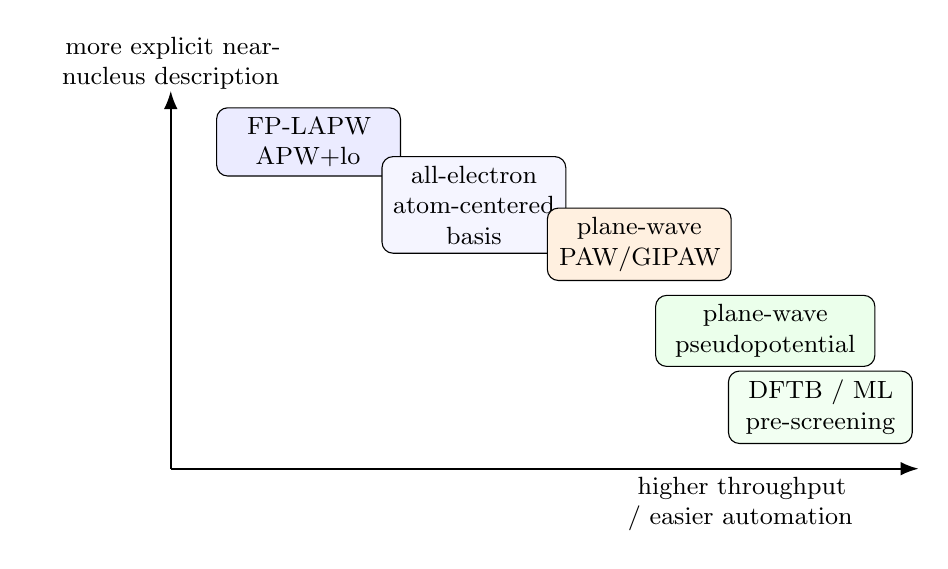
\begin{tikzpicture}[x=1cm,y=1cm,>=Latex,
  method/.style={draw,rounded corners,align=center,font=\small,minimum height=0.72cm,text width=2.1cm}
]
  \draw[->,thick] (0,0) -- (9.5,0);
  \draw[->,thick] (0,0) -- (0,4.8);
  \node[align=center,font=\small,text width=4.2cm] at (7.25,-0.45) {higher throughput / easier automation};
  \node[align=center,font=\small,text width=3.4cm] at (0,5.15) {more explicit near-nucleus description};

  \node[method,fill=blue!8] at (1.75,4.15) {FP-LAPW\\APW+lo};
  \node[method,fill=blue!4] at (3.85,3.35) {all-electron\\atom-centered basis};
  \node[method,fill=orange!12] at (5.95,2.85) {plane-wave\\PAW/GIPAW};
  \node[method,text width=2.55cm,fill=green!8] at (7.55,1.75) {plane-wave\\pseudopotential};
  \node[method,fill=green!5] at (8.25,0.78) {DFTB / ML\\pre-screening};
\end{tikzpicture}
\caption{A qualitative accuracy-speed map for local tensor calculations.  It is a guide to thinking, not a universal ranking: a well-converged PAW calculation can beat a poorly converged all-electron calculation, and structure or functional errors can dominate both.}
\label{fig:methodmap}
\end{figure}

\section{Focusing on ABINIT PAW and Elk FP-LAPW}

After the broad map, we now return to the two backends most relevant to the current package design.  ABINIT and Elk are useful examples because they represent two different but complementary philosophies.  ABINIT with PAW is attractive for automated, high-throughput, package-integrated EFG calculations.  Elk is attractive as an all-electron benchmark path when the result is important or surprising.  This distinction should be presented as a workflow choice, not as a claim that one code is always ``right'' and the other is always ``approximate.''

\begin{table}[H]
\centering
\small
\begin{tabularx}{\textwidth}{L{0.18\textwidth}Y Y}
\toprule
 & \textbf{ABINIT PAW plane-wave workflow} & \textbf{Elk all-electron FP-LAPW workflow} \\
\midrule
Core idea & Smooth plane waves plus PAW reconstruction near nuclei. & All-electron basis: radial functions in muffin tins plus plane waves in the interstitial. \\
Best role in a package & Default backend for routine estimates, convergence scans, automated structure-to-tensor conversion, and high-throughput site assignment. & Reference backend for selected cases, publication checks, heavy or core-sensitive nuclei, and cases where PAW datasets disagree. \\
Speed & Usually fast enough for routine structure screening and many-site calculations.  EFG output adds little cost after the SCF density exists. & Usually slower for the same cell and less forgiving of default parameters. \\
Automation & Well suited to scripted workflows from CIF/POSCAR to parsed tensor output. & Automatable, but robust automation needs more expert rules for muffin tins, local orbitals, and basis settings. \\
Near-nucleus accuracy & Often good if PAW datasets are high quality and convergence is tested. & Strong all-electron reference for near-nuclear properties. \\
Main knobs & Plane-wave cutoff, PAW dataset, semicore choice, k-point grid, smearing, SCF tolerance, relaxation criteria. & Muffin-tin radii, $\RMT K_{\max}$, local orbitals, angular-momentum cutoffs, k-points, core/valence treatment, SCF tolerance. \\
Main failure modes & Soft or inappropriate PAW dataset, missing semicore states, insufficient cutoff, wrong structure, fragile magnetism, finite-temperature/disorder effects. & More setup complexity, poor muffin-tin choices, basis linearization issues, slow convergence, high cost for large cells. \\
\bottomrule
\end{tabularx}
\caption{ABINIT and Elk as two useful ends of a practical workflow spectrum.}
\label{tab:abinit-elk}
\end{table}

A sensible documentation policy is:
\begin{quote}
Use ABINIT/PAW for routine workflows, convergence studies, and initial quadrupolar predictions.  Use Elk/FP-LAPW as a reference calculation when ABINIT results are surprising, when PAW dataset choice matters, when semicore or heavy-element effects may be important, or when a publication requires a stronger cross-check.
\end{quote}

\subsection{Illustrative ABINIT EFG workflow}

A minimal ABINIT EFG calculation is a normal ground-state PAW calculation with nuclear EFG output enabled.  Exact values are system-dependent; the fragment below is illustrative, not a universal default.

\begin{lstlisting}[language={},caption={Illustrative ABINIT EFG input fragment.}]
# Ground-state PAW calculation for a periodic crystal
usepaw 1
ixc -101130             # example PBE convention; check ABINIT version
ecut 30.0               # converge this for the PAW datasets and EFG
ngkpt 4 4 4             # converge this for the material
nstep 100
toldfe 1.0d-10

# Request nuclear-site electric-field gradients
nucefg 2                # EFG plus quadrupole couplings
quadmom 0.02044 ...     # nuclear Q values, one per atom type
\end{lstlisting}

Important package-level notes:
\begin{itemize}
\item The EFG request is meaningful in the PAW formalism.
\item The quadrupole moment values affect reported couplings, not the raw EFG tensor itself.
\item The EFG post-processing is cheap compared with the SCF calculation, but the SCF density must be tightly converged.
\item Parsers should preserve tensor components, principal values, eigenvectors, units, atom labels, and symmetry-equivalent site information.
\end{itemize}

\subsection{Illustrative ABINIT phonon and response workflow}

The ABINIT EFG example above is a ground-state property workflow.  Phonons, dielectric response, elastic constants, and related derivative properties use a different ABINIT pattern.  After a well-converged ground-state calculation, ABINIT response-function datasets compute first-order wavefunctions and energy derivatives for selected perturbations.  Those derivatives are written to a DDB file; DDB files can be merged with MRGDDB; ANADDB then performs the heavier analysis step.\cite{ABINIT_RESPFN,ABINIT_ANADDB}

A schematic example is:

\begin{lstlisting}[language={},caption={Schematic ABINIT response/ANADDB flow, not a complete input deck.}]
# 1. Ground-state SCF calculation: converge density and wavefunctions.
# 2. DFPT response calculations, for example:
optdriver 1       # response-function driver
rfphon 1          # atomic-displacement perturbations for phonons
rfelfd 2          # electric-field response when dielectric/Born data are needed
rfstrs 1          # strain response when elastic data are needed
# ... choose q-points, atoms, directions, convergence, and output DDB files ...

# 3. Optional: merge derivative databases from several perturbations/q-points.
#    mrgddb < mrgddb.files

# 4. Analyze the derivative database.
#    anaddb < anaddb.files
# Outputs may include phonon bands, interatomic force constants,
# dielectric/Born tensors, elastic/piezoelectric data, and thermodynamics.
\end{lstlisting}

A documentation note for beginners should make clear that the DDB is not itself the final phonon band structure or thermal model.  It is the derivative database from which ANADDB constructs those outputs.  This is analogous to saving a linearized small-signal model after finding a DC operating point in circuit simulation: the saved derivative information can be reused for multiple analyses, but the user still needs to specify which analysis is desired.

\subsection{Illustrative Elk EFG workflow}

In Elk, the usual idea is to run a converged ground-state all-electron calculation and request the electric-field-gradient task.  The exact input syntax and recommended parameters should be checked against the Elk version used by the package.

\begin{lstlisting}[language={},caption={Illustrative Elk task fragment.}]
tasks
  0     : ground-state calculation
  115   : electric field gradient at nuclear sites

# Parameters such as rgkmax, gmaxvr, lmaxapw,
# muffin-tin radii, local orbitals, and k-points
# must be tested for the target tensor.
\end{lstlisting}

For Elk, the most important documentation point is not the short task request; it is convergence.  Users need to understand that all-electron accuracy comes with additional basis parameters.  Muffin-tin radii, local orbitals, angular-momentum cutoffs, and $\RMT K_{\max}$ can all affect the result.

\section{Accuracy-speed trade-offs}

The preceding sections separate three sources of variation: the electronic method, the structural model, and the software implementation.  The practical question for users is how much extra cost is justified for a given prediction.  The answer depends on whether the calculation is being used for a quick search window, a site assignment, or a publication-quality comparison.

\subsection{What controls speed?}

The cost of a DFT calculation is controlled by several factors:
\begin{itemize}
\item number of atoms and valence electrons;
\item number of basis functions or grid points;
\item number of k-points;
\item number of empty bands, meaning unoccupied Kohn-Sham states needed for some response and excited-state calculations;
\item exchange-correlation functional, especially hybrid functionals;
\item metallic versus insulating occupation behavior;
\item number of SCF iterations and geometry-optimization steps;
\item whether spin polarization, spin-orbit coupling, noncollinear magnetism, or finite-temperature sampling is included.
\end{itemize}
Direct diagonalization has a steep scaling with system size, often described informally as cubic scaling in the number of electronic states.  Modern codes use many algorithmic tricks, but the qualitative message remains: doubling the number of atoms can cost much more than twice as much.

\subsection{Implementation, parallelism, and math libraries}

The preceding list describes the physics and numerical size of the problem.  The actual wall-clock time, meaning the time a user waits for a job to finish, also depends strongly on how the DFT code was compiled and launched.  A DFT executable is a high-performance numerical program, not just a formula evaluator.  Two runs with the same input file can differ substantially if one uses a serial executable and another uses an optimized parallel build.

The first performance concept to define is the \emph{Message Passing Interface} (MPI): a standard way to run many cooperating processes, often across several compute nodes.  In a DFT code, MPI ranks may divide work over k-points, bands, spins, plane-wave coefficients, real-space grids, perturbations, or independent images such as geometry-optimization replicas.  A second concept is \emph{OpenMP}, a shared-memory threading interface in which one process starts multiple threads, usually within a single node.  Many production runs use a hybrid layout, for example several MPI ranks per node and several OpenMP threads per rank.  The best layout is code-, problem-, and machine-dependent; using more processors does not guarantee a proportional speedup because of communication, synchronization, load imbalance, memory bandwidth, input/output, and serial parts of the algorithm.  ABINIT's own parallelism documentation emphasizes that only certain parts of a calculation parallelize efficiently and that scaling must be tested on the target machine.\cite{ABINIT_BASEPAR,ABINIT_PARALLEL_TOPIC}

The second performance concept is the numerical library stack.  \emph{Basic Linear Algebra Subprograms} (BLAS) are standard routines for vector and matrix operations, while \emph{Linear Algebra PACKage} (LAPACK) provides standard dense linear-algebra routines such as eigenvalue solvers.  Optimized implementations, for example OpenBLAS, Intel oneAPI Math Kernel Library (MKL), AMD Optimizing CPU Libraries (AOCL), Cray LibSci, or IBM Engineering and Scientific Subroutine Library (ESSL), can be much faster than a generic reference implementation on the same hardware.  \emph{Scalable LAPACK} (ScaLAPACK) and \emph{Eigenvalue SoLvers for Petaflop Applications} (ELPA) provide distributed-memory linear algebra for some large MPI jobs.  Plane-wave codes also spend significant time in \emph{fast Fourier transforms} (FFTs), so FFT libraries such as FFTW or vendor FFT libraries may matter.  ABINIT's build and linear-algebra documentation explicitly treats MPI, BLAS, LAPACK, ScaLAPACK, ELPA, FFTW, OpenMP, and vendor math libraries as important build choices.\cite{ABINIT_BUILD,ABINIT_LINALG,ABINIT_BASEPAR}  The Elk project likewise advertises MPI, OpenMP, and hybrid MPI/OpenMP parallelization as part of the code.\cite{ElkSite}

For package documentation, the useful beginner message is practical rather than heroic.  Use the DFT executable supplied by a trusted cluster module, package manager, or reproducible build system when possible; check that it is linked to appropriate BLAS/LAPACK/FFT libraries; and run a small scaling test for the class of problem the package will generate.  A scaling test compares, for example, 1 MPI rank with many threads, many MPI ranks with 1 thread each, and a hybrid MPI-plus-thread layout.  Users should avoid \emph{oversubscription}, which means accidentally asking for more software threads than physical CPU cores, for example by combining many MPI ranks, OpenMP threads, and multithreaded BLAS threads at the same time.  Environment variables such as \texttt{OMP\_NUM\_THREADS}, \texttt{OPENBLAS\_NUM\_THREADS}, and \texttt{MKL\_NUM\_THREADS} are commonly used to control thread counts, and OpenBLAS documents \texttt{OPENBLAS\_NUM\_THREADS} as one way to control its threading in multi-threaded applications.\cite{OpenBLAS}  The exact policy should still follow the local cluster documentation.

This is especially relevant for relaxation, phonons, and ensemble calculations.  A single EFG calculation may be dominated by one SCF run, but a finite-displacement phonon workflow, an ABINIT DFPT q-point grid, or an MD/thermal-disorder ensemble may require tens to hundreds of related electronic-structure calculations.  These workflows often expose extra parallelism: different displacements, q-points, snapshots, spin configurations, or candidate structures can be distributed across jobs even when one individual SCF calculation no longer scales well.

\subsection{What controls accuracy?}

Accuracy is not controlled by a single slider.  The largest errors may come from the electronic approximation, the structure, the basis, the pseudopotential/PAW dataset, or the finite-temperature model.  For EFGs, the structure and near-nucleus charge density are especially important.  A beautifully converged calculation on the wrong CIF structure can be worse than a modest calculation on the correct structure.

\begin{table}[H]
\centering
\small
\begin{tabularx}{\textwidth}{L{0.22\textwidth}Y Y}
\toprule
\textbf{Choice} & \textbf{Usually faster} & \textbf{Usually more accurate / safer} \\
\midrule
Structure & Use CIF as-is & Validate symmetry, resolve disorder, check hydrogens, use temperature-matched structure, relax carefully \\
Basis & Lower cutoff or smaller local basis & Converge target tensor with cutoff/basis size and grid settings \\
Core treatment & Soft pseudopotential; fewer valence states & Harder PAW, semicore in valence, or all-electron benchmark \\
Brillouin-zone sampling & Coarse k-point grid & Converge $\Vzz$, $\etaEFG$, and any magnetic quantities versus k-points \\
Functional & PBE/PBEsol GGA & Test dispersion, DFT+$U$, meta-GGA, hybrid, or benchmark family where needed \\
Temperature & Single static 0 K-like structure & Temperature-matched structure, phonon or MD ensemble, tensor averaging \\
DFT backend & Automated PAW plane-wave workflow & PAW convergence plus all-electron cross-check for critical sites \\
Runtime stack & Default serial or workstation launch & Benchmark MPI/OpenMP layout and use optimized BLAS/LAPACK/FFT libraries appropriate to the machine \\
\bottomrule
\end{tabularx}
\caption{Common speed-accuracy trade-offs.  The right column is not always necessary; it is the direction to move when a prediction is important or questionable.}
\label{tab:tradeoffs}
\end{table}

\subsection{Recommended convergence target}

For routine package use, a pragmatic convergence target might be that $\CQ$ changes by less than 1--5\% under reasonable increases in cutoff, k-point mesh, and basis quality.  For publication-quality comparison to experiment, the target may need to be tighter, and structural uncertainty should be included.  Reporting three decimal places for a frequency is misleading if the structure, functional, or PAW dataset shifts the result by 10\%.

\section{Practical accuracy pitfalls}

\subsection{Numerical convergence}

A DFT calculation can have a well-converged total energy while a local tensor is still moving by several percent.  Convergence studies should track the actual output quantities: $\Vzz$, $\etaEFG$, tensor orientation, $\CQ$, and derived frequencies.  For magnetic systems, also track magnetic moments and total-energy differences between spin states.

\subsection{Exchange-correlation functional}

GGA functionals such as PBE are common because they are robust and relatively inexpensive.  However, EFGs are sensitive to local bonding and electronic anisotropy.  Molecular crystals, hydrogen-bonded systems, correlated $d$ or $f$ electrons, charge-transfer systems, and van der Waals solids may require more care.  Dispersion corrections, PBEsol, meta-GGAs, DFT+$U$, hybrid functionals, or molecular-cluster corrections can improve some systems, but there is no universal best choice.

\subsection{Core, semicore, and relativistic treatment}

EFGs depend strongly on the charge distribution near the nucleus.  In PAW or pseudopotential calculations, ask:
\begin{itemize}
\item Are semicore states included as valence when needed?
\item Is the PAW radius too large or too soft for a near-nuclear tensor property?
\item Are scalar-relativistic or spin-orbit effects important?
\item Is the chosen nuclear quadrupole moment $Q$ current and isotope-specific?
\end{itemize}
For heavy nuclei, relativistic effects and core treatment can become limiting.  For light nuclei, local bonding and hydrogen positions may dominate.

\subsection{Crystal structure quality and CIF issues}

For many NQR problems, the largest error is not the electronic solver; it is the structure.  A CIF file is a crystallographic data-exchange file, not a guarantee of a DFT-ready atomistic model.  Common issues include:
\begin{itemize}
\item hydrogen atoms missing or placed by riding models in X-ray structures;
\item partial occupancy or disorder represented statistically rather than as a single explicit configuration;
\item thermal displacement parameters that describe motion, not static coordinates;
\item coordinates measured at a temperature different from the NQR experiment;
\item insufficient coordinate precision in old or manually transcribed CIF files;
\item symmetry operations that generate overlapping atoms if interpreted incorrectly;
\item missing solvent, wrong protonation state, wrong charge state, or ambiguous atom labels;
\item isotope information absent from atom labels.
\end{itemize}
The practical recommendation is to treat CIF ingestion as a preprocessing and validation step, not merely a file conversion.

\subsection{Structural relaxation and finite-temperature effects}

Section~\ref{sec:relax-phonons} treated this topic in detail because it is often the dominant source of uncertainty.  The short version is that a static DFT calculation gives a tensor for one structural model.  Real NMR/NQR spectra may reflect thermal expansion, phonons, molecular librations, dynamic disorder, slow conformer exchange, or static disorder.  Package documentation should therefore distinguish clearly between an unrelaxed tensor, a fixed-cell relaxed tensor, a fully relaxed tensor, and a phonon/MD/disorder-averaged tensor.

A practical warning is that relaxation can improve local chemistry while also moving away from the experimental temperature.  Phonons can reveal unstable structures, provide thermal displacement patterns, and estimate tensor averaging, but they add additional convergence and sampling choices.  Users should not be forced into a single policy; instead, the package should record the policy used and make it visible in the output metadata.

\subsection{Magnetism, metals, defects, and surfaces}

\begin{description}
\item[Metals] Smearing and dense k-point sampling can strongly affect convergence and local tensors.
\item[Magnetic materials] Different spin states can have different charge densities and therefore different local tensors.  Check the magnetic order.
\item[Spin-orbit coupling] Important for heavy elements, magnetic anisotropy, $g$ tensors, and some hyperfine terms.  It increases cost and convergence complexity.
\item[Defects and surfaces] Supercell size, charge corrections, vacuum thickness, and electrostatic boundary conditions can dominate the error.
\item[Disordered molecular solids] One crystallographic site may correspond to a distribution of local environments.  A single EFG tensor may be an oversimplification.
\end{description}

\section{Recommended practical workflow}

\subsection{Generic structure-to-property workflow}

\begin{enumerate}
\item Identify the physical question: site assignment, frequency search window, tensor orientation, finite-temperature shift, or benchmark comparison.
\item Choose the structure source and validate it: polymorph, temperature, protonation, disorder, hydrogen positions, charge state, and isotope labels.
\item Choose a DFT method appropriate to the question: routine PAW, all-electron benchmark, molecular cluster, or ensemble workflow.
\item Run SCF convergence tests for the target property, not only for total energy.
\item If needed, relax the structure using a documented policy: no relaxation, hydrogen-only correction, fixed-cell internal relaxation, or full relaxation.
\item Decide whether a finite-temperature treatment is needed.  For sensitive cases, generate phonon, MD, strain, or disorder snapshots and compute tensors for each configuration.
\item Extract tensors and metadata.  Store raw tensor components, principal values, eigenvectors, units, code convention, structural policy, thermal policy, and nuclear data.
\item Convert to spin-Hamiltonian parameters only after tensor parsing and convention checks.
\item Compare with experiment, known compounds, or a second DFT method when the result is important.
\end{enumerate}

\subsection{Convergence report template}

For reproducible predictions, the package should encourage users to save a small convergence report:
\begin{center}
\small
\begin{tabularx}{\textwidth}{@{}L{0.23\textwidth}Y@{}}
\toprule
\textbf{Quantity} & \textbf{What to record} \\
\midrule
Structure & source, temperature, relaxation choice, disorder choices, hydrogen policy \\
DFT code & code, version, pseudopotential/PAW dataset or all-electron settings \\
Build and launch & MPI ranks, OpenMP threads, BLAS/LAPACK/FFT libraries, ScaLAPACK/ELPA use, processor/GPU type if relevant, and job-scheduler settings \\
Functional & PBE, PBEsol, LDA, DFT+$U$, dispersion correction, hybrid, etc. \\
Basis & cutoff, grid settings, local basis, or FP-LAPW basis parameters \\
Sampling & k-point mesh, smearing method, electronic supercell size \\
SCF & energy, density, force, and stress convergence criteria \\
Thermal model & none, phonon snapshots, AIMD snapshots, quasi-harmonic expansion, disorder ensemble; for ABINIT, DDB/ANADDB provenance \\
EFG result & full tensor, principal values, $\Vzz$, $\etaEFG$, tensor orientation \\
Nuclear data & isotope, quadrupole moment $Q$, source of $Q$ \\
Derived spectrum & $\CQ$, zero-field transition frequencies, sign convention \\
Sensitivity & changes under tighter cutoff/k-mesh, alternative PAW, or all-electron check \\
\bottomrule
\end{tabularx}
\end{center}

\section{Implementation notes for a spin-dynamics package}

The interface between DFT and spin dynamics should avoid throwing away information.  Recommended internal data fields include:
\begin{itemize}
\item atom label, element, isotope, crystallographic Wyckoff/site label if available;
\item Cartesian EFG tensor in the crystal frame;
\item principal values and principal-axis rotation matrix;
\item $\Vzz$, $\etaEFG$, sign convention, ordering convention, and units;
\item nuclear quadrupole moment $Q$ and its source;
\item $\CQ$ and zero-field transition frequencies;
\item multiplicity of symmetry-equivalent sites;
\item DFT metadata: code, version, functional, basis/cutoff, k-points, convergence thresholds, structure source;
\item performance metadata: executable or module name, MPI ranks, OpenMP threads, BLAS/LAPACK/FFT library choices, and any relevant scheduler or environment variables;
\item preprocessing metadata: CIF warnings, hydrogen policy, relaxation policy, phonon/MD/disorder averaging policy, temperature assumptions, and ABINIT DDB/ANADDB provenance when derivative databases are used.
\end{itemize}

For propagation, it is often better to reconstruct $\mathcal H_Q$ from the full tensor than from a scalar frequency.  This avoids ambiguity when adding RF fields, Zeeman terms, strain perturbations, rotations, powder averaging, or time-dependent EFG modulation.

\section{What accuracy should users expect?}

There is no universal error bar.  A beginner-facing summary is:
\begin{itemize}
\item \textbf{Trends and site assignments:} often reliable when structures are good and convergence has been tested.
\item \textbf{Absolute $\CQ$ values:} errors of several percent to tens of percent are possible, especially for poor structures, difficult bonding, heavy elements, or correlated materials.
\item \textbf{$\etaEFG$:} often more sensitive than $\Vzz$ because it depends on differences between smaller principal components.
\item \textbf{Frequency search aid:} DFT is very useful for narrowing a search window and identifying inequivalent sites, but should not be treated as a substitute for experimental calibration.
\item \textbf{Benchmark path:} if the prediction is critical, compare ABINIT/PAW against Elk/FP-LAPW or another all-electron code, check alternative PAW datasets, test structural relaxation choices, and compare to known compounds in the same chemical family.
\end{itemize}

\section{Glossary}

\begin{longtable}{@{}L{0.18\textwidth}L{0.76\textwidth}@{}}
\toprule
\textbf{Term} & \textbf{Meaning} \\
\midrule
\endhead
1WF & First-order wavefunction, the linear electronic-response quantity computed in many DFPT calculations. \\
2DTE / 3DTE & Second or third derivative of the total energy.  ABINIT stores such derivative information in DDB files for later analysis. \\
ABINIT & Open-source plane-wave DFT code.  In this context, useful with PAW for automated EFG calculations and with DDB/ANADDB workflows for phonons and response properties. \\
AIMD & Ab initio molecular dynamics: molecular dynamics in which forces are computed from electronic-structure calculations during the trajectory. \\
AOCL & AMD Optimizing CPU Libraries, a vendor numerical-library suite for AMD processors. \\
ANADDB & ABINIT's Analysis of Derivative DataBase utility; it post-processes DDB files into phonon, dielectric, elastic, thermodynamic, and related response quantities. \\
All-electron & A method that treats core and valence electrons explicitly rather than replacing the core by a pseudopotential. \\
APW & Augmented plane wave, a basis family using atom-centered functions near nuclei and plane waves between atoms. \\
ASE & Atomic Simulation Environment, a Python ecosystem often used to build and automate atomistic simulations. \\
ASR & Acoustic sum rule, a translational-invariance condition often imposed when post-processing phonon force constants. \\
BLAS & Basic Linear Algebra Subprograms, standard low-level dense vector and matrix routines used by many DFT codes. \\
Born effective charge & A response tensor describing how macroscopic polarization changes when an atom is displaced. \\
Born-Oppenheimer approximation & Separation of electronic and nuclear motion because electrons are much lighter and faster than nuclei. \\
Brillouin zone (BZ) & Primitive cell of reciprocal space; k-point grids sample it. \\
$\CQ$ & Quadrupole coupling constant, often $eQ\Vzz/h$.  Check sign and unit conventions. \\
CIF & Crystallographic Information File.  A common exchange format for crystal structures; not automatically a DFT-ready model. \\
DDB & Derivative DataBase, an ABINIT file containing total-energy derivatives from response-function calculations. \\
DFT & Density-functional theory, an electronic-structure method based on the electron density. \\
DFT+$U$ & A correction often used for localized $d$ or $f$ electrons in strongly correlated systems. \\
DFPT & Density-functional perturbation theory, used for response properties such as phonons, dielectric tensors, Born charges, and related quantities. \\
Dielectric tensor & Tensor describing electric polarization response to an applied electric field. \\
Dynamical matrix & Mass-weighted force-constant matrix whose eigenvalues give squared phonon frequencies in the harmonic approximation. \\
DOS & Density of states, the number of electronic states per energy interval. \\
EFG & Electric-field-gradient tensor $V_{ij}$ at a nuclear site. \\
Elk & Open-source all-electron full-potential LAPW/APW+lo code.  Useful as a high-accuracy reference for EFGs. \\
ELPA & Eigenvalue SoLvers for Petaflop Applications, a library for distributed-memory eigenvalue problems in large electronic-structure calculations. \\
EPR/ESR & Electron paramagnetic resonance/electron spin resonance. \\
ESSL & IBM Engineering and Scientific Subroutine Library, a vendor-optimized numerical-library suite. \\
FFT & Fast Fourier transform, an algorithm used heavily in plane-wave DFT. \\
FFTW & Fastest Fourier Transform in the West, a widely used open-source FFT library. \\
Finite displacement & Numerical derivative method in which atoms are displaced slightly and forces or properties are recomputed. \\
Force & Derivative of total energy with respect to atomic displacement; used for structural relaxation and phonons. \\
FP-LAPW & Full-potential linearized augmented plane wave, an all-electron method with no shape approximation to the potential. \\
GAPW & Gaussian and augmented plane wave, a CP2K method that improves near-core reconstruction relative to standard GPW. \\
GGA & Generalized-gradient approximation, a class of exchange-correlation functional depending on density and density gradient. \\
GIPAW & Gauge-including projector augmented wave.  Used especially for NMR magnetic shielding and other magnetic-response properties in periodic systems. \\
GPW & Gaussian and plane wave, the mixed-basis method used in CP2K's Quickstep module. \\
Hamiltonian & Operator governing spin energy levels and time evolution.  DFT supplies parameters for some Hamiltonian terms. \\
Harmonic approximation & Approximation that the energy near equilibrium is quadratic in atomic displacements; the basis of standard phonon calculations. \\
Hybrid functional & Exchange-correlation functional including a fraction of exact exchange.  Often more expensive, sometimes more accurate. \\
k-point & A reciprocal-space sampling point.  More k-points are needed for smaller cells, metals, and high-accuracy calculations. \\
Kohn-Sham equations & Effective one-electron equations solved self-consistently in practical DFT. \\
LAPW & Linearized augmented plane wave. \\
LAPACK & Linear Algebra PACKage, a standard library interface for dense numerical linear algebra. \\
LCAO & Linear combination of atomic orbitals. \\
LDA & Local-density approximation, an early class of exchange-correlation functional. \\
LibSci & Cray/HPE scientific-library suite containing optimized numerical routines on many supercomputers. \\
MD & Molecular dynamics, a simulation of atomic motion through time. \\
MKL & Intel oneAPI Math Kernel Library, a vendor numerical-library suite for BLAS, LAPACK, FFT, and related routines. \\
MPI & Message Passing Interface, a standard for parallel programs composed of communicating processes, often across compute nodes. \\
MRGDDB & ABINIT utility for merging multiple DDB files before ANADDB analysis. \\
Muffin tin & Atom-centered region in LAPW/APW methods where radial basis functions are used. \\
NAO & Numeric atom-centered orbital. \\
NMR & Nuclear magnetic resonance. \\
NQR & Nuclear quadrupole resonance, usually zero-field transitions driven by the quadrupolar Hamiltonian. \\
OpenBLAS & Open-source optimized implementation of BLAS. \\
OpenMP & Shared-memory threading interface commonly used inside one compute node. \\
PAW & Projector augmented wave, an efficient method that reconstructs all-electron-like behavior near nuclei. \\
PBE & Perdew-Burke-Ernzerhof GGA functional, a common default in plane-wave DFT. \\
PBEsol & PBE revised for solids; sometimes improves lattice constants. \\
PBC & Periodic boundary conditions. \\
Phonon & A crystal vibrational normal mode.  Phonons are used to study dynamic stability, thermal motion, and temperature-dependent averaging. \\
POSCAR & Common VASP structure file format containing lattice vectors and atomic positions. \\
Pseudopotential & Effective potential replacing core electrons and the bare nucleus to make calculations tractable. \\
Quasi-harmonic approximation & Approximation that combines harmonic phonons with volume-dependent frequencies to estimate thermal expansion and finite-temperature thermodynamics. \\
RF & Radio-frequency; in spin dynamics, often refers to applied oscillating magnetic fields used for excitation and control. \\
SCF & Self-consistent field, the iterative loop that makes the input density and output density agree. \\
ScaLAPACK & Scalable LAPACK, a distributed-memory linear-algebra library based on MPI. \\
Semicore & Electrons below the nominal valence shell that may still affect bonding or near-nuclear properties. \\
Smearing & Smooth occupation method used to stabilize metallic or small-gap calculations. \\
SOC & Spin-orbit coupling, important for heavy elements and many magnetic properties. \\
Stress & Derivative of total energy with respect to cell strain; used for cell relaxation. \\
$\Vzz$ & Largest-magnitude principal component of the EFG tensor by common NMR convention. \\
Wyckoff position & Symmetry label for crystallographically equivalent sites in a space group. \\
XC & Exchange-correlation, the approximate part of DFT describing quantum many-body effects beyond classical electrostatics. \\
XYZ & Simple coordinate file format listing atoms and Cartesian positions; it usually lacks periodic cell information. \\
Zeeman interaction & Interaction of a magnetic moment with an applied magnetic field. \\
$\etaEFG$ & EFG asymmetry parameter, usually $(V_{xx}-V_{yy})/V_{zz}$ after a specified ordering convention. \\
\bottomrule
\end{longtable}

\section{Short checklist for package users}

\begin{enumerate}
\item Start from a structure that corresponds to the material, polymorph, protonation state, and temperature of interest.
\item Inspect and validate the structure before running DFT; treat CIF/POSCAR ingestion as model construction, not merely file conversion.
\item Choose the DFT method according to the property: routine PAW for throughput, all-electron for selected benchmarks.
\item For EFGs, use PAW/GIPAW or all-electron methods; do not rely on a plain pseudopotential result without reconstruction.
\item Converge $\Vzz$, $\etaEFG$, tensor orientation, and derived frequencies, not just total energy.
\item For nontrivial jobs, record and test the launch configuration: MPI ranks, OpenMP threads, BLAS/LAPACK/FFT libraries, and any thread-count environment variables.
\item Preserve the full tensor, orientation, structural model, and thermal model in the spin-dynamics input.
\item Treat DFT-predicted NQR frequencies as search aids unless benchmarked against experiment or a higher-confidence calculation.
\item For surprising or important results, cross-check with a harder PAW dataset, a different functional, fixed-cell relaxation, phonon or MD sampling, and/or Elk or another all-electron method.
\end{enumerate}

\section*{Acknowledgment of scope}

This note intentionally omits many details of electronic-structure theory: variational-principle derivations, formal density-functional theorems, advanced exchange-correlation development, many-body perturbation theory, relativistic electronic structure, anharmonic lattice dynamics, and detailed code-specific input syntax.  The goal is to give NMR/NQR and electrical-engineering users enough conceptual footing to run, parse, and critique DFT-derived solid-state parameters without treating the DFT engine as a black box.

\begin{thebibliography}{99}
\small

\bibitem{HohenbergKohn1964}
P.~Hohenberg and W.~Kohn, ``Inhomogeneous electron gas,'' \emph{Physical Review}, vol.~136, pp.~B864--B871, 1964.

\bibitem{KohnSham1965}
W.~Kohn and L.~J.~Sham, ``Self-consistent equations including exchange and correlation effects,'' \emph{Physical Review}, vol.~140, pp.~A1133--A1138, 1965.

\bibitem{PBE1996}
J.~P.~Perdew, K.~Burke, and M.~Ernzerhof, ``Generalized gradient approximation made simple,'' \emph{Physical Review Letters}, vol.~77, pp.~3865--3868, 1996.

\bibitem{Blochl1994}
P.~E.~Blochl, ``Projector augmented-wave method,'' \emph{Physical Review B}, vol.~50, pp.~17953--17979, 1994.

\bibitem{Petrilli1998}
H.~M.~Petrilli, P.~E.~Blochl, P.~Blaha, and K.~Schwarz, ``Electric-field-gradient calculations using the projector augmented wave method,'' \emph{Physical Review B}, vol.~57, pp.~14690--14697, 1998.

\bibitem{Profeta2003}
M.~Profeta, F.~Mauri, and C.~J.~Pickard, ``Accurate first principles prediction of $^{17}$O NMR parameters in SiO$_2$: Assignment of the zeolite ferrierite spectrum,'' \emph{Journal of the American Chemical Society}, vol.~125, pp.~541--548, 2003.

\bibitem{PickardMauri2001}
C.~J.~Pickard and F.~Mauri, ``All-electron magnetic response with pseudopotentials: NMR chemical shifts,'' \emph{Physical Review B}, vol.~63, 245101, 2001.

\bibitem{Charpentier2011}
T.~Charpentier, ``The PAW/GIPAW approach for computing NMR parameters: A new dimension added to NMR study of solids,'' \emph{Solid State Nuclear Magnetic Resonance}, vol.~40, pp.~1--20, 2011.

\bibitem{ABINIT_EFG}
The ABINIT Group, ``EFG,'' ABINIT documentation, version 10.6.7, 2026.  Available: \url{https://docs.abinit.org/topics/EFG/}

\bibitem{ABINIT_NUC}
The ABINIT Group, ``Properties at the nucleus,'' ABINIT tutorial documentation, 2026.  Available: \url{https://docs.abinit.org/tutorial/nuc/}

\bibitem{Gonze2020}
X.~Gonze \emph{et al.}, ``The ABINIT project: Impact, environment and recent developments,'' \emph{Computer Physics Communications}, vol.~248, 107042, 2020.

\bibitem{ElkSite}
J.~K.~Dewhurst, S.~Sharma, and collaborators, ``The Elk Code,'' official project site.  Available: \url{https://elk.sourceforge.io/}

\bibitem{ElkManual}
J.~K.~Dewhurst, S.~Sharma, and collaborators, \emph{The Elk Code Manual}.  Available: \url{https://elk.sourceforge.io/elk.pdf}

\bibitem{QEsite}
Quantum ESPRESSO Foundation, ``Quantum ESPRESSO,'' official project site. Available: \url{https://www.quantum-espresso.org/}

\bibitem{Giannozzi2017}
P.~Giannozzi \emph{et al.}, ``Advanced capabilities for materials modelling with Quantum ESPRESSO,'' \emph{Journal of Physics: Condensed Matter}, vol.~29, 465901, 2017.

\bibitem{VASP_LEFG}
The VASP Wiki, ``LEFG,'' 2025. Available: \url{https://vasp.at/wiki/LEFG}

\bibitem{VASP_QUAD}
The VASP Wiki, ``QUAD\_EFG,'' 2025. Available: \url{https://vasp.at/wiki/QUAD_EFG}

\bibitem{Kresse1996}
G.~Kresse and J.~Furthmuller, ``Efficient iterative schemes for ab initio total-energy calculations using a plane-wave basis set,'' \emph{Physical Review B}, vol.~54, pp.~11169--11186, 1996.

\bibitem{CASTEP_NMR}
CASTEP developers, ``Solid-state NMR,'' CASTEP documentation. Available: \url{https://www.castep.org/features/capabilities/solid-state-nmr}

\bibitem{Clark2005}
S.~J.~Clark \emph{et al.}, ``First principles methods using CASTEP,'' \emph{Zeitschrift fur Kristallographie}, vol.~220, pp.~567--570, 2005.

\bibitem{CP2K_GPW}
CP2K developers, ``Gaussian Plane Wave Method,'' CP2K documentation. Available: \url{https://www.cp2k.org/gpw}

\bibitem{VandeVondele2005}
J.~VandeVondele \emph{et al.}, ``Quickstep: Fast and accurate density functional calculations using a mixed Gaussian and plane waves approach,'' \emph{Computer Physics Communications}, vol.~167, pp.~103--128, 2005.

\bibitem{GPAWsite}
GPAW developers, ``GPAW: DFT and beyond within the projector-augmented wave method,'' documentation. Available: \url{https://gpaw.readthedocs.io/}

\bibitem{Enkovaara2010}
J.~Enkovaara \emph{et al.}, ``Electronic structure calculations with GPAW: A real-space implementation of the projector augmented-wave method,'' \emph{Journal of Physics: Condensed Matter}, vol.~22, 253202, 2010.

\bibitem{WIEN2kSite}
P.~Blaha, K.~Schwarz, and collaborators, ``WIEN2k,'' official project site. Available: \url{https://susi.theochem.tuwien.ac.at/}

\bibitem{Schwarz2003}
K.~Schwarz, P.~Blaha, and G.~K.~H.~Madsen, ``Electronic structure calculations of solids using the WIEN2k package for material sciences,'' \emph{Computer Physics Communications}, vol.~147, pp.~71--76, 2002.

\bibitem{ExcitingSite}
The exciting code developers, ``exciting,'' official project site. Available: \url{https://exciting-code.org/home/about/exciting}

\bibitem{Gulans2014}
A.~Gulans \emph{et al.}, ``exciting: a full-potential all-electron package implementing density-functional theory and many-body perturbation theory,'' \emph{Journal of Physics: Condensed Matter}, vol.~26, 363202, 2014.

\bibitem{FHIaimsSite}
FHI-aims developers, ``FHI-aims: all-electron electronic structure theory with numeric atom-centered orbitals,'' official site. Available: \url{https://fhi-aims.org/}

\bibitem{Blum2009}
V.~Blum \emph{et al.}, ``Ab initio molecular simulations with numeric atom-centered orbitals,'' \emph{Computer Physics Communications}, vol.~180, pp.~2175--2196, 2009.

\bibitem{SIESTA_Docs}
SIESTA developers, ``A First Encounter with SIESTA,'' SIESTA documentation. Available: \url{https://docs.siesta-project.org/}

\bibitem{Soler2002}
J.~M.~Soler \emph{et al.}, ``The SIESTA method for ab initio order-N materials simulation,'' \emph{Journal of Physics: Condensed Matter}, vol.~14, pp.~2745--2779, 2002.

\bibitem{CRYSTALsite}
CRYSTAL developers, ``CRYSTAL,'' official project site. Available: \url{https://www.crystal.unito.it/}

\bibitem{Dovesi2018}
R.~Dovesi \emph{et al.}, ``Quantum-mechanical condensed matter simulations with CRYSTAL,'' \emph{WIREs Computational Molecular Science}, vol.~8, e1360, 2018.

\bibitem{Hartman2021}
J.~D.~Hartman, A.~Mathews, and J.~K.~Harper, ``Fast and accurate electric field gradient calculations in molecular solids with density functional theory,'' \emph{Frontiers in Chemistry}, vol.~9, article 751711, 2021.

\bibitem{Choudhary2020}
K.~Choudhary, J.~N.~Ansari, I.~I.~Mazin, and K.~L.~Sauer, ``Density functional theory based electric field gradient database,'' \emph{Scientific Data}, vol.~7, article 362, 2020.

\bibitem{Reina2025}
J.~V.~Reina \emph{et al.}, ``The EFG Rosetta Stone: translating between DFT calculations and solid state NMR experiments,'' \emph{Faraday Discussions}, 2025, doi:10.1039/D4FD00075G.

\bibitem{Pyykko2008}
P.~Pyykko, ``Year-2008 nuclear quadrupole moments,'' \emph{Molecular Physics}, vol.~106, pp.~1965--1974, 2008.

\bibitem{Pyykko2018}
P.~Pyykko, ``Year-2017 nuclear quadrupole moments,'' \emph{Molecular Physics}, vol.~116, pp.~1328--1338, 2018.

\bibitem{Baroni2001}
S.~Baroni, S.~de Gironcoli, A.~Dal Corso, and P.~Giannozzi, ``Phonons and related crystal properties from density-functional perturbation theory,'' \emph{Reviews of Modern Physics}, vol.~73, pp.~515--562, 2001.

\bibitem{Togo2015}
A.~Togo and I.~Tanaka, ``First principles phonon calculations in materials science,'' \emph{Scripta Materialia}, vol.~108, pp.~1--5, 2015.

\bibitem{PhonopyDocs}
A.~Togo and collaborators, ``Phonopy documentation,'' official documentation. Available: \url{https://phonopy.github.io/phonopy/}

\bibitem{QEPhononGuide}
Quantum ESPRESSO Foundation, ``PHonon User's Guide,'' official documentation. Available: \url{https://www.quantum-espresso.org/Doc/ph_user_guide/}

\bibitem{ABINIT_DFPTTopic}
The ABINIT Group, ``DFPT,'' ABINIT documentation. Available: \url{https://docs.abinit.org/topics/DFPT/}

\bibitem{ABINIT_RESPFN}
The ABINIT Group, ``Response functions,'' ABINIT documentation. Available: \url{https://docs.abinit.org/guide/respfn/}

\bibitem{ABINIT_ANADDB}
The ABINIT Group, ``The anaddb utility,'' ABINIT documentation. Available: \url{https://docs.abinit.org/guide/anaddb/}

\bibitem{ABINIT_PHONONS}
The ABINIT Group, ``Phonons,'' ABINIT documentation. Available: \url{https://docs.abinit.org/topics/Phonons/}

\bibitem{ABINIT_DFPT}
The ABINIT Group, ``Response-function tutorials,'' ABINIT documentation. Available: \url{https://docs.abinit.org/tutorial/}

\bibitem{ABINIT_BUILD}
The ABINIT Group, ``How to build ABINIT using the Autotools,'' ABINIT documentation. Available: \url{https://docs.abinit.org/tutorial/abinit_build/}

\bibitem{ABINIT_LINALG}
The ABINIT Group, ``Configuring linear algebra,'' ABINIT documentation. Available: \url{https://www.abinit.org/linear_algebra.html}

\bibitem{ABINIT_PARALLEL_TOPIC}
The ABINIT Group, ``Parallelism,'' ABINIT documentation. Available: \url{https://docs.abinit.org/topics/parallelism/}

\bibitem{ABINIT_BASEPAR}
The ABINIT Group, ``Basic parallelization in ABINIT,'' ABINIT documentation. Available: \url{https://docs.abinit.org/tutorial/basepar/}

\bibitem{OpenBLAS}
OpenMathLib, ``OpenBLAS: an optimized BLAS library,'' official project documentation. Available: \url{https://www.openmathlib.org/OpenBLAS/}

\bibitem{Slichter}
C.~P.~Slichter, \emph{Principles of Magnetic Resonance}, 3rd ed.  Springer, 1990.

\end{thebibliography}

\end{document}
